% Revisión 23-11-2026: versión principal en español con IEEEtran A4.
% Cambios: IMRyD, comparación IoT/Flutter/Xamarin, evidencia Android, transferencia y anexos.
\documentclass[conference,a4paper]{IEEEtran}
\usepackage[T1]{fontenc}
\usepackage[spanish,es-tabla,es-nodecimaldot]{babel}
\usepackage{amsmath,booktabs,graphicx}
\usepackage[hidelinks]{hyperref}
\usepackage{xurl}
\graphicspath{{figures/}}
\renewcommand{\abstractname}{Resumen}
\renewcommand{\IEEEkeywordsname}{Palabras clave}
\hypersetup{
  pdftitle={UCRA: diagnóstico visual y asistencia móvil para reparar prendas},
  pdfauthor={Lopez Arela, Ower Frank; Zegarra Puma, Mauricio Eduardo; Huamani Chañi, Diego Oswaldo},
  pdflang={es}
}

\title{UCRA: diagnóstico visual con abstención y asistencia móvil para la reparación de prendas}
\author{\IEEEauthorblockN{Lopez Arela, Ower Frank}
\and \IEEEauthorblockN{Zegarra Puma, Mauricio Eduardo}
\and \IEEEauthorblockN{Huamani Chañi, Diego Oswaldo}}

\begin{document}
\maketitle
\begin{abstract}
ReparaAI es una aplicación Android de asistencia a la reparación textil. UCRA combina control de calidad de imagen, localización selectiva de agujeros, confirmación del usuario, consulta de procedimientos con fuente y registro local. Se compararon cuatro detectores con 407 vistas de 406 prendas de CISUTAC, de las cuales 61 se reservaron para prueba. El modelo por mosaicos mostró 18 candidatos y acertó en 8 vistas con intersección sobre unión (IoU) de al menos 0,25. Siete vistas alcanzaron IoU de 0,50. La precisión entre propuestas fue 44,4\% con abstención y 19,7\% al mostrar una propuesta en cada vista. En 358 vistas externas de tela de FabriD, el modelo congelado localizó 0 de 77 vistas con agujeros y mostró 14 candidatos en 88 vistas con anotación vacía. La inferencia y el registro funcionan sin conexión. Los resultados delimitan el uso experimental del detector y motivan una validación independiente en prendas cotidianas.
\end{abstract}
\begin{IEEEkeywords}
reparación textil, Flutter, visión por computador, abstención, recuperación de procedimientos
\end{IEEEkeywords}

\section{Introducción}

Reparar una prenda exige identificar el daño, comprobar el tipo de tela y elegir una técnica que la persona pueda ejecutar. Diddi y Yan encontraron que la falta de habilidades, el tiempo y el coste de servicios profesionales dificultan la reparación entre consumidores encuestados \cite{diddi2019}. La Agencia Europea de Medio Ambiente identifica la reparación y el uso prolongado como estrategias de circularidad textil \cite{eea}. La necesidad analizada es la orientación para reparaciones domésticas de prendas comunes. El estudio no midió demanda comercial ni ahorro ambiental.

El objetivo general es diseñar y evaluar un flujo móvil que conecte una observación visual con un procedimiento con fuente y permita continuar la reparación sin conexión. Los objetivos específicos son implementar captura y control de calidad, comparar métodos de localización por prenda, medir el efecto de abstenerse y verificar el guardado del progreso y del resultado. Se estudian dos hipótesis de ingeniería. La primera plantea que una red con mapas de centros aumenta la fracción de vistas localizadas frente a un bosque de ventanas fijas. La segunda plantea que un umbral de abstención aumenta la precisión de las propuestas a costa de cobertura.

\subsection{Antecedentes y alcance}
DeepFashion2 aporta categorías y máscaras de prendas \cite{ge2019}. El conjunto de segunda mano de RISE y colaboradores incluye atributos de condición \cite{nauman}. Garment Condition Holes de CISUTAC incluye anotaciones espaciales de agujeros \cite{cisutac}. FabricSpotDefect ofrece supervisión sobre manchas en otro dominio de captura \cite{fabricspot}. Los detectores por puntos aportan una formulación para estimar centros y tamaños \cite{zhou2019}. La clasificación selectiva relaciona riesgo y cobertura \cite{geifman2017}, y la calibración exige evidencia sobre la correspondencia entre una puntuación y la probabilidad de acierto \cite{guo2017}. La recuperación aumentada de texto permite condicionar la generación a fuentes \cite{lewis2020}. UCRA emplea un catálogo curado y reglas deterministas en su línea base de asistencia.

Una \emph{propuesta} es una región sugerida por el detector. El \emph{daño observado} es la identificación del usuario tras inspeccionar la prenda. El \emph{resultado} es lo que la persona reporta al cerrar la sesión. El sistema registra cada dato con su origen.

\section{Métodos}

\subsection{Análisis de requisitos y selección tecnológica}
Se analizaron las tareas desde la captura hasta el cierre de la reparación. Se derivaron requisitos verificables para foto, recomendación y persistencia. Por ejemplo, una imagen deficiente debe llevar a repetir la captura. Una tela desconocida debe retener la recomendación. La sesión debe recuperar el último paso guardado al reiniciar el proceso. Los instrumentos empleados fueron el dataset y sus anotaciones, métricas calculadas en Python, pruebas de Flutter, el emulador Android, la interfaz de accesibilidad de Android y una lectura de SQLite para verificar persistencia.

Flutter ofrece una interfaz común con acceso a servicios nativos \cite{flutter}. Se eligió para integrar captura y ejecución de ONNX en Android con interfaz bilingüe y un proyecto iOS. Xamarin fue una alternativa estudiada durante el curso. Microsoft cerró su soporte en mayo de 2024 y dirige la migración hacia .NET MAUI \cite{xamarin}. En IoT, el NIST distingue una interfaz de red y un transductor en el dispositivo \cite{nist8259}. En ReparaAI, la cámara es el sensor y el teléfono procesa la información localmente. Un nodo de inspección conectado sería una extensión de IoT que requeriría su propia integración y pruebas.

\subsection{Diseño del sistema}
Flutter orquesta la selección de fotos, el procesamiento, el detector ONNX, el catálogo y SQLite. La resolución mínima es 384 píxeles por eje. La app comprueba luminancia media entre 0,07 y 0,96 y energía laplaciana de al menos 0,00012. El catálogo filtra por daño, tela y equipo e incluye cuatro técnicas con fuente \cite{guides,patches}. Los planes y sus referencias se guardan por sesión. Las fotos se exportan a JPEG sin EXIF. Un control permite comparar el antes y después visualmente. En GitHub Pages \cite{githubpages}, el mismo flujo ejecuta ONNX Runtime Web mediante WebAssembly en el navegador \cite{onnxweb} y conserva el diario en IndexedDB. La Fig.~\ref{fig:arquitectura} resume el flujo.

\begin{figure}[!t]
\centering
\setlength{\tabcolsep}{2pt}
\begin{tabular}{@{}ccc@{}}
  \fbox{Cámara o galería} & $\to$ & \fbox{Control de calidad} \\
  && $\downarrow$ \\
  && \fbox{Detección ONNX} \\
  && $\downarrow$ \\
  && \fbox{Candidato o abstención} \\
  && $\downarrow$ \\
  \fbox{Catálogo con fuentes} & $\to$ & \fbox{Confirmación y guía} \\
  && $\downarrow$ \\
  && \fbox{Historial local SQLite}
\end{tabular}
\caption{Flujo de análisis y reparación. La confirmación del usuario precede a la selección del procedimiento.}
\label{fig:arquitectura}
\end{figure}

\begin{figure*}[!t]
\centering
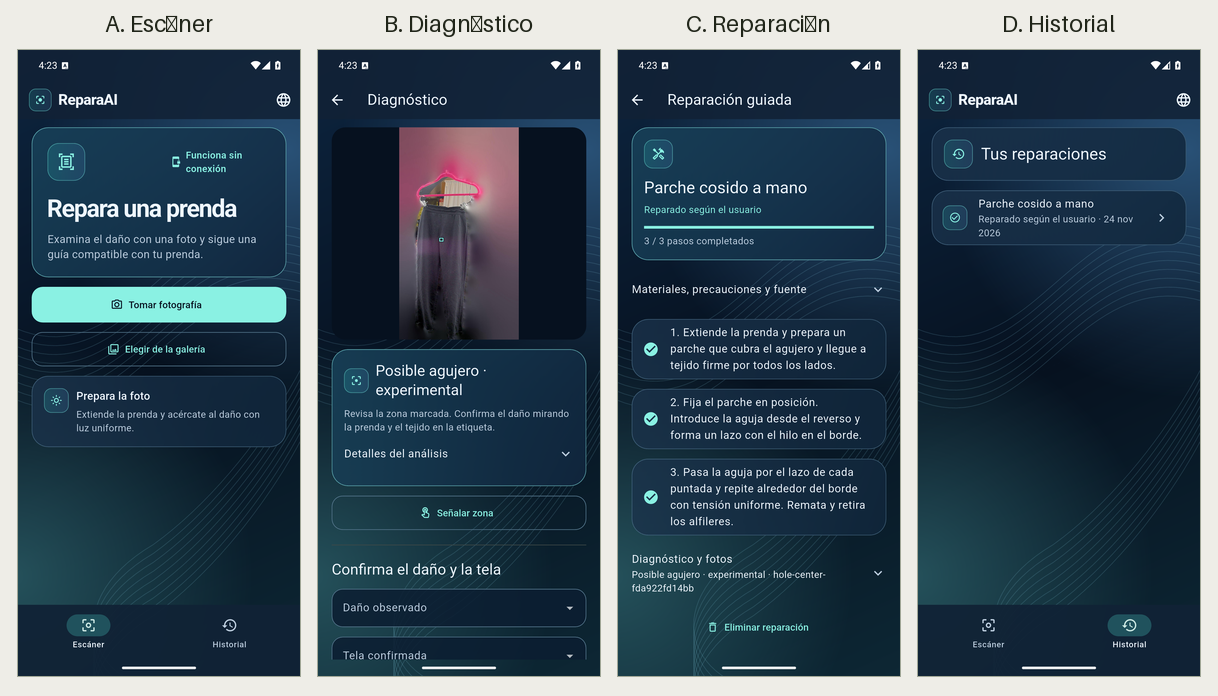
\includegraphics[width=.88\textwidth]{flujo_android.png}
\caption{Capturas de ReparaAI en el emulador Android. La fotografía procedente de CISUTAC y Wargön Innovation se muestra bajo CC BY 4.0 \cite{cisutac}. La sesión documenta una prueba de software.}
\label{fig:capturas}
\end{figure*}

\subsection{Dataset y modelos}
La revisión fijada de CISUTAC contiene 761 exportaciones con anotaciones pareadas y fondos procesados \cite{cisutac}. Se conservó la variante de mayor resolución por vista, se transformaron tres registros poligonales en sus cajas envolventes antes de deduplicar y se verificaron las coordenadas. La partición con semilla 104 utilizó el identificador de prenda del archivo para evitar transferir vistas de una prenda entre grupos. La Tabla~\ref{tab:datos} muestra los recuentos. La revisión, licencia y script de adquisición están en el repositorio.

\begin{table}[!t]
\centering
\caption{Distribución después de deduplicar por vista}
\label{tab:datos}
\begin{tabular}{lrrr}
\toprule
Partición & Prendas & Vistas & Agujeros \\
\midrule
Entrenamiento & 284 & 285 & 571 \\
Validación & 61 & 61 & 115 \\
Prueba & 61 & 61 & 99 \\
\bottomrule
\end{tabular}
\end{table}

Las líneas base usan ventanas cuadradas de 8, 16, 32 y 64 píxeles en una cuadrícula de $384\times384$, con avance de media ventana. Sus descriptores representan luminancia, contraste, gradiente y escala. La regresión logística pondera clases. El bosque usa 32 árboles, profundidad máxima 10 y al menos 12 muestras por hoja. Se entrenaron con 998 ventanas positivas y 27,448 negativas según el solapamiento con anotaciones.

La red convolucional predice un mapa de centros con paso 4 y estima tamaño y desplazamiento para cada centro. Combina pérdida focal y regresión $L_1$ suavizada. La variante de vista completa usa $384\times384$ píxeles. La versión por mosaicos usa una cuadrícula de $1152\times1152$, selecciona la mejor propuesta entre 16 recortes solapados y devuelve la caja en coordenadas globales. Ambas redes se entrenaron durante 24 épocas con AdamW en una NVIDIA GeForce RTX 4060 Ti. Se emplearon volteos, variación de luz y recortes. La versión por mosaicos también toma recortes de fondo durante el entrenamiento. El modelo desplegado contiene 166,085 parámetros y pesa alrededor de 654 KiB.

\subsection{Métricas y prueba funcional}
Sea $\hat b$ la caja de mayor puntuación y $B$ el conjunto de cajas anotadas en una vista. Se considera acierto cuando $\max_{b\in B}\operatorname{IoU}(\hat b,b) \geq u$. Se analizan $u=0{,}25$ y $u=0{,}50$. La cobertura divide los candidatos mostrados entre todas las vistas. La precisión selectiva divide los aciertos entre los candidatos mostrados. La fracción localizada divide los aciertos entre las vistas positivas. Se ajustó el umbral en validación mediante $F_{0.5}$. Los intervalos percentiles al 95\% se estimaron con 1000 remuestreos por prenda.

La prueba funcional reproduce una sesión completa en un emulador Android 16 en modo avión con un archivo de prueba seleccionado de CISUTAC. Verifica el selector de galería, el candidato, la confirmación, el plan con fuente, el avance, el reinicio, la evidencia y el resultado persistido. Este caso seleccionado comprueba la integración del software. Las pantallas de la Fig.~\ref{fig:capturas} muestran el recorrido ejecutado.

Para explorar un cambio de dominio, se ejecutó el ONNX móvil sobre las 358 vistas de prueba oficiales de FabriD v1 \cite{fabrid}, sin entrenamiento ni ajuste de umbral. Se separaron vistas con polígonos de agujero, vistas con otras clases anotadas y vistas con archivo de anotación vacío. Los polígonos se transformaron en cajas envolventes. Se reporta cobertura por grupo e intervalos de Wilson descriptivos por vista.

Para estudiar la búsqueda guiada, se limitó la selección del centro a una ventana de 20\% por eje alrededor de una marca. En CISUTAC se simuló la marca a partir del centro de la mayor anotación, con desplazamientos uniformes de hasta seis puntos porcentuales por eje. Se conservó el mismo ONNX y el mismo umbral. Este diseño mide el efecto de una marca aproximadamente correcta en una prueba controlada.

\section{Resultados}

\begin{table}[!t]
\centering
\caption{Localización en las 61 vistas reservadas}
\label{tab:metricas}
\setlength{\tabcolsep}{4pt}
\begin{tabular}{lrrrr}
\toprule
Modelo & Mostr. & $\geq0{,}25$ & $\geq0{,}50$ & Precisión (IC 95\%) \\
\midrule
Logística & 59 & 1 & 0 & 1,7 (0,0--5,2) \\
Bosque & 53 & 3 & 2 & 5,7 (0,0--12,5) \\
CNN completa & 40 & 2 & 0 & 5,0 (0,0--12,9) \\
CNN mosaicos & 18 & 8 & 7 & 44,4 (21,4--68,8) \\
\bottomrule
\end{tabular}
\end{table}

La Tabla~\ref{tab:metricas} presenta los resultados con umbrales elegidos en validación. La red de vista completa localizó dos vistas con IoU de 0,25, frente a tres del bosque. La variante por mosaicos localizó ocho. La diferencia de la fracción localizada entre mosaicos y bosque fue de 8,2 puntos porcentuales (IC pareado del 95\% entre 0,0 y 16,4). La cobertura del detector desplegado fue 29,5\%.

Al mostrar la propuesta de cada vista, los mosaicos acertaron en 12 de 61 casos (19,7\%). Con abstención acertaron en 8 de 18 (44,4\%). El umbral suprimió 43 candidatos y cuatro aciertos. El control de calidad dejó pasar las vistas procesadas por el proveedor, de modo que su efecto adicional fue nulo en esta muestra. La Fig.~\ref{fig:riesgo} visualiza el intercambio entre cobertura y error.

En el caso seleccionado para integración, la caja del emulador obtuvo IoU de 0,699 con la anotación y el procesamiento tomó 4,04 s en una ejecución de depuración. Se verificaron tres pasos guardados y la persistencia de ambas fotos tras reiniciar. El tiempo ilustra la ejecución en el emulador. La latencia en teléfonos físicos permanece por medir.

\begin{table}[!t]
\centering
\caption{Comparación del mismo ONNX en las 61 vistas de CISUTAC}
\label{tab:guiada}
\setlength{\tabcolsep}{3pt}
\begin{tabular}{lrrrr}
\toprule
Búsqueda & Mostr. & IoU $\geq$ 0,25 & IoU $\geq$ 0,50 & Prec. \\
\midrule
Completa & 18 & 8 & 7 & 44,4\% \\
Marca simulada & 16 & 11 & 8 & 68,8\% \\
\bottomrule
\end{tabular}
\end{table}

La Tabla~\ref{tab:guiada} muestra el incremento de aciertos de 8 a 11 con una zona acotada. La marca simulada usó la anotación de referencia y representa ayuda manual idealizada. Las mejoras no estiman la precisión que lograrían participantes sin acceso a las anotaciones.

\subsection{Transferencia a FabriD}
El detector mostró 16 candidatos en 77 vistas con agujeros, sin coincidencias a IoU de 0,25. Emitió 14 candidatos en 88 vistas con anotación vacía (15,9\%, IC del 95\% de 9,7 a 25,0) y 55 en 193 vistas con otros defectos (28,5\%, IC del 95\% de 22,6 a 35,2). La identidad física de cada pieza no consta. Los puntos e intervalos resumen el archivo de prueba de telas. La anotación vacía se interpreta según la exportación y no equivale a una inspección física independiente.

\begin{figure}[!t]
\centering
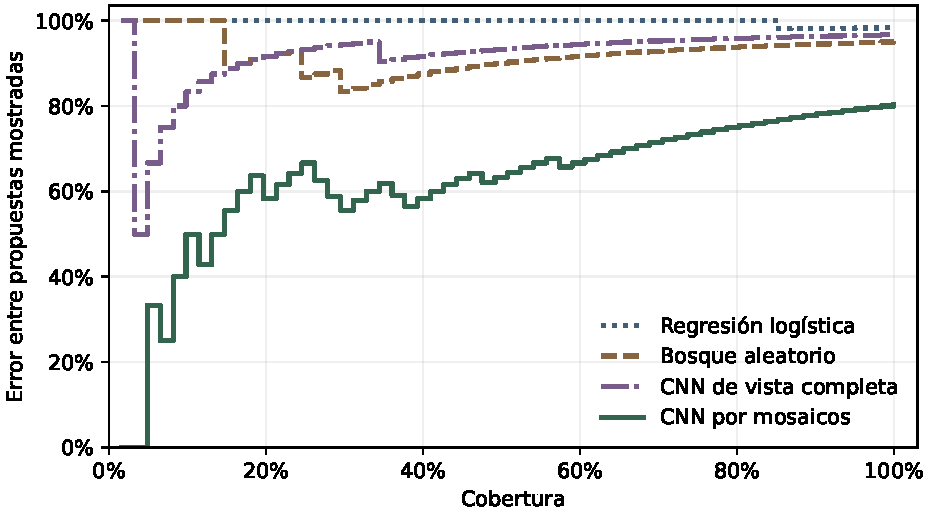
\includegraphics[width=\columnwidth]{riesgo_cobertura.pdf}
\caption{Error de localización entre propuestas mostradas, por cobertura. Cada escalón corresponde a un umbral de puntuación.}
\label{fig:riesgo}
\end{figure}

\section{Discusión}
La comparación sugiere que un detector que conserva mayor detalle espacial puede encontrar daños que desaparecen al escalar toda la imagen. El cambio de resolución coincide con cambios en los recortes de entrenamiento y con más propuestas durante la inferencia. Por ello el efecto aislado de la resolución sigue abierto. La reducción observada del error con abstención es descriptiva y debe replicarse con una prueba externa. Incluso con el umbral seleccionado, diez candidatos del modelo desplegado no alcanzaron IoU de 0,25.

Frente a trabajos centrados en la descripción de la prenda \cite{ge2019} o en la condición para clasificación de residuos \cite{nauman,cisutac}, UCRA conserva la relación entre una región propuesta, la confirmación del usuario y la guía utilizada. La integración móvil aporta trazabilidad al ensayo. La estrategia de recomendación cubre pocos casos y requiere revisión independiente de compatibilidad.

El benchmark de prendas de CISUTAC contiene fondos procesados y carece de vistas negativas verificadas. FabriD aporta un dominio externo de telas con anotaciones distintas y exhibe una pérdida de localización. Ambas evaluaciones dejan abierta la especificidad, calibración y transferencia a fotografías de prendas tomadas con un celular. Una caja principal por vista no permite estimar detección de múltiples defectos. La app guarda un resultado declarado por el usuario. El estudio carece de mediciones de resistencia de costuras, pruebas de uso con participantes y desempeño en teléfonos físicos. La investigación siguiente debe incluir prendas íntegras, daños ambiguos, variación de iluminación, negativos difíciles y revisión doble de anotaciones. La recuperación requiere casos revisados por especialistas.

\section{Conclusiones}
ReparaAI une detección selectiva, contexto confirmado, procedimientos con fuente y persistencia sin conexión. El piloto cuantifica la baja localización inicial y el intercambio entre aciertos y cobertura. La asistencia manual permite consultar una guía cuando la detección se abstiene. La evidencia disponible sustenta una validación técnica inicial del flujo y delimita las pruebas necesarias para establecer su fiabilidad.

\appendices
\section{Reproducibilidad y trazabilidad}
El repositorio \href{https://github.com/OwerLopez/RepairAI}{OwerLopez/RepairAI} incluye adquisición, entrenamiento, tablas generadas, validación de ONNX, catálogo y prueba Android. Se puede abrir la \href{https://owerlopez.github.io/RepairAI/}{aplicación web} y descargar el \href{https://github.com/OwerLopez/RepairAI/releases/tag/v0.2.0}{APK de pruebas}. La foto de integración se identifica por archivo. Los metadatos del detector registran SHA-256. El protocolo de anotación y los resultados están en los anexos del repositorio.

\section{Registro de revisión}
La revisión del 23 de noviembre de 2026 incorpora formato IEEE A4, contenido IMRyD en español, análisis de IoT y Xamarin, comparación agrupada y transferencia a FabriD. El código fuente incluye comentarios de revisión. Afiliaciones, autor de correspondencia, declaraciones de intereses y funciones CRediT quedan por confirmar por el equipo.

\IEEEtriggeratref{9}
\bibliographystyle{IEEEtran}
\bibliography{references}
\end{document}
